\documentclass[12pt,a4paper]{article}
\usepackage[utf8]{inputenc}
\usepackage{amsmath}
\usepackage{amsfonts}
\usepackage{amssymb}
\usepackage{graphicx}
\author{Kyle Latino}
\begin{document}

Kyle Latino


\begin{center}
\textbf{\Large A page in Latex}
\end{center}

Here are some useful mathematic formulas.

$(a+b)^2=a^2+2ab+b^2$

$$ a^2-b^2=(a+b)(a-b) $$

\[ f(x)=e^x+2x+1 \]

\begin{equation}\label{eq1}
f(x)=e^x+2x+1
\end{equation}

Differentiating (\ref{eq1}), we get
\begin{equation}\label{eq2}
f'(x)=e^x+2
\end{equation}

\begin{equation}\label{eq3}
f''(x)=e^x
\end{equation}

On integration (\ref{eq3}), becomes
\[ \int f(x)\, dx =e^x +C \]

\[ \int_0^1 e^x\, dx = \left. e^x \right|_0^1 = e-1 \]

\noindent\hrulefill

Here is a table.

\begin{tabular}{ccc}
Left & Center & Right \\ 
4 & 5 & 6 \\ 
7 & 8 & 9 \\ 
10 & 11 & 12 \\ 
13 & 14 & 15 \\ 
\end{tabular} 

\begin{center}
\begin{tabular}{|c|c|c|}
\hline 
1 & 2 & 3 \\ 
\hline 
4 & 5 & 6 \\ 
\hline 
7 & 8 & 9 \\ 
\hline 
10 & 11 & 12 \\ 
\hline 
13 & 14 & 15 \\ 
\hline 
\end{tabular} 
\end{center}
 
\begin{center}
\rotatebox{270}{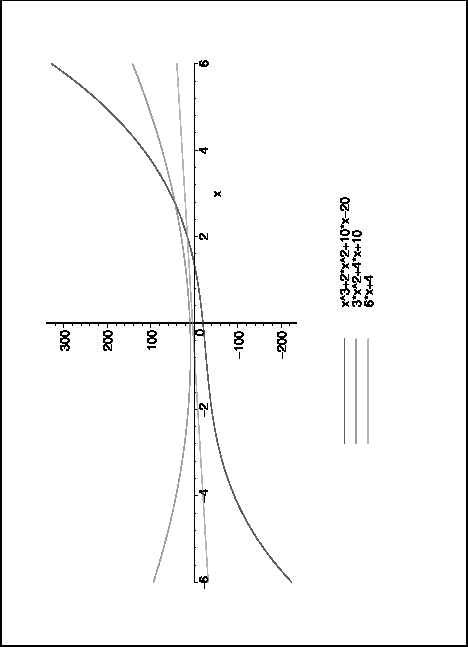
\includegraphics[scale=0.5]{plot1.jpg} }
\end{center}

\end{document}